\subsection{Estaciones ferroviarias}
    \label{sec:platform}
    
    Las estaciones ferroviarias son las zonas donde las formaciones pueden detenerse para que los pasajeros puedan descender y nuevos pasajeros puedan abordar. En función del tamaño de las formaciones y la geografía del lugar, las plataformas desde donde ascienden y descienden los pasajeros pueden estar elevadas con respecto al suelo o a ras del mismo. El largo de las plataformas también depende de la cantidad de coches de las formaciones.
    
    Como puede verse en la Figura \ref{fig:estacion_1}, las estaciones ferroviarias incluyen no solo a las plataformas, sino que también pueden centralizar el control de varias operaciones logísticas como la asignación de rutas. No obstante, en este trabajo nos referiremos a las estaciones como plataformas indistintamente.
    
        \begin{figure}[!h]
            \centering
            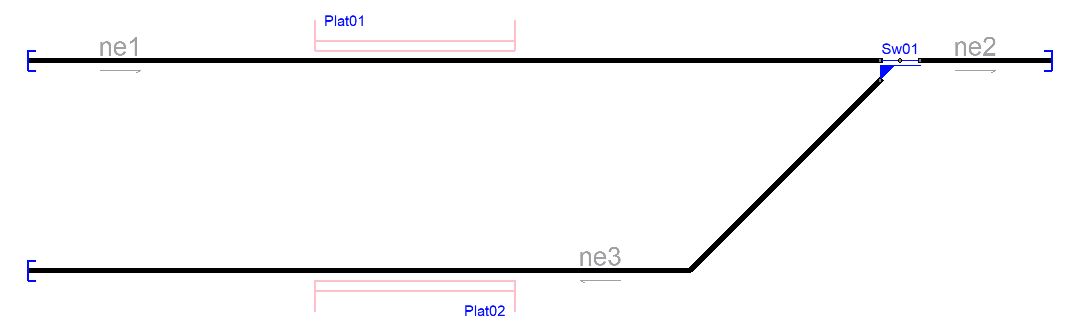
\includegraphics[width=1\textwidth]{Figuras/Platform.png}
            \centering\caption{Estación de doble plataforma.}
            \label{fig:estacion_1}
        \end{figure}
    
    Las estaciones de mayor complejidad o de mayor convergencia de ramales suelen concentrar el control de la estación donde se encuentran y varias estaciones vecinas. Las estaciones terminales, a menudo, pueden incluso tener control total de varios ramales completos.

    En el Código \ref{lst:platform_1} se pueden ver la implementación de la clase platform de las plataformas ilustradas en la Figura \ref{fig:estacion_1}. Esta clase se encuentra dentro de la clase infrastructure, que a su vez contiene a la clase functionalInfrastructure. La misma incluye atributos como la altura, el nombre asignado que se visualiza en la Figura \ref{fig:estacion_1} y el netElement al que se encuentran asociadas cada una de las plataformas.

    \begin{lstlisting}[language = XML, caption = Clase Platform , label = {lst:platform_1}]
    <platforms>
        <platform id="plf3" height="0">
            <name name="Plat01" language="en"/>
            <linearLocation id="plf3_lloc01" applicationDirection="both">
                <associatedNetElement keepsOrientation="true" netElementRef="ne1"/>
            </linearLocation>
            <designator register="_Example" entry="PLATFORM Plat01"/>
            <length type="physical" value="0" validForDirection="both"/>
        </platform>
        <platform id="plf6" height="0">
            <name name="Plat02" language="en"/>
            <linearLocation id="plf6_lloc01" applicationDirection="both">
                <associatedNetElement keepsOrientation="true" netElementRef="ne3"/>
            </linearLocation>
            <designator register="_Example" entry="PLATFORM Plat02"/>
            <length type="physical" value="0" validForDirection="both"/>
        </platform>
    </platforms>
    \end{lstlisting}

    Los datos relativos a la características físicas como el largo y el ancho la encontramos dentro de la clase visualization, dentro de la clase infrastructureVisualizations, como se puede ver en el Código \ref{lst:platform_2}.

    \begin{lstlisting}[language = XML, caption = Clase visualization , label = {lst:platform_2}]
    <spotElementProjection refersToElement="plf3" id="vis01_sep4">
        <name name="Plat01" language="en"/>
        <coordinate x="-125.455" y="-240.000"/>
    </spotElementProjection>
    <spotElementProjection refersToElement="plf6" id="vis01_sep5">
        <name name="Plat02" language="en"/>
        <coordinate x="-125.454" y="-30.000"/>
    </spotElementProjection>
    \end{lstlisting}

    Conocer las dimensiones del elemento físico que representa esta clase es fundamental a la hora de analizar el impacto de este elemento en la red y donde se deberían asignar las señales ferroviarias.